%priprava posamezne ure
%tukaj zaporedoma napisemo{st. zaporedne ure}{datum}{naslov}{poglavje}{oblika dela}{pripomocki}
\begin{priprava}{}{}{Odvod}{Uvod}{frontalna}{tabla}

\didopomba{Začnemo pa takoj po poglavju limite funkcije, brez omenjanja besede ``odvod''. Šele po omembi lahko na začetek napišemo naslov novega poglavja: ``ODVOD''}

Uvodna motivacija (graf finančnega stanja) \didopomba{To govoriš in zraven rišeš graf}:

Leta 2030 magistriraš in začneš svoje podjetje, na začetku imaš 15.000 €. V treh letih profitiraš na 100.000 € in ti ni treba več biti menedžer sam sebi, ampak enega najameš. Nadajnje stanje financ pa opiše ta graf \didopomba{in dorišeš potem dolino, na dnu se menja menedžer, gre navzgor, na vrhu nov menedžer, ker je ta drugi šel v penzijo, pa gre spet navzdol \ldots}.

\begin{figure*}[h]
    \centering
    \includegraphics[width=0.6\textwidth]{slike/menedžer.png}
\end{figure*}

Kateri menedžer je boljši? \didopomba{tisti, po katerem graf začne naraščati}. Torej ocena za menedžerja je to naraščanje/padanje ($ M_1 $ dobi oceno $ -2, M_2 $ oceno $ + 1{,}5 $, čeprav je pri prvem več financ. \didopomba{Še sebe oceniš z $ + 3 $, za primerjavo s ta dobrim menedžerjem, da pride do izraza razlika v koeficientih})

Kako pa bi lahko izračunali to ``strmino''? \didopomba{Koeficient neke premice. (če ne vejo, greš z naslednjim primerom naprej, tam pa bojo ja pogruntali) Narišeš še en primer s premicami -- pot v odvisnosti od časa za avto, tekača in polža, torej tre premice iz izhodišča z različnim koeficientom -- katera je bolj strma? Od avta, ampak kaj na premici ti pove strmino? $ \rightarrow $ koeficient.}

Ponovimo koeficient premice ( $ k = \frac{\Delta y}{\Delta x} = \frac{y_2 - y_1}{x_2 - x_1} $ \didopomba{s slikco!})

Torej pri primeru z avtom, tekačem in polžem je strmejša tista premica, ki ima višji koeficient. Kaj pa pri menedžerjih? Tam nimamo premic, ampak je graf ukrivljen. \didopomba{naj probajo sami pridet na idejo tangente. Fora pa je ista -- višji koeficient tangente, boljši je menedžer (primerjava sebe in $ M_2 $)}.

Naslednji problem je, kako izračunati koeficient tangente na ukrivljen graf. \didopomba{tu pa zdaj začnemo na splošno risati in namignemo na sekanto, uporabi GEOGEBRO!}

\newpage

\begin{figure*}[h]
    \centering
    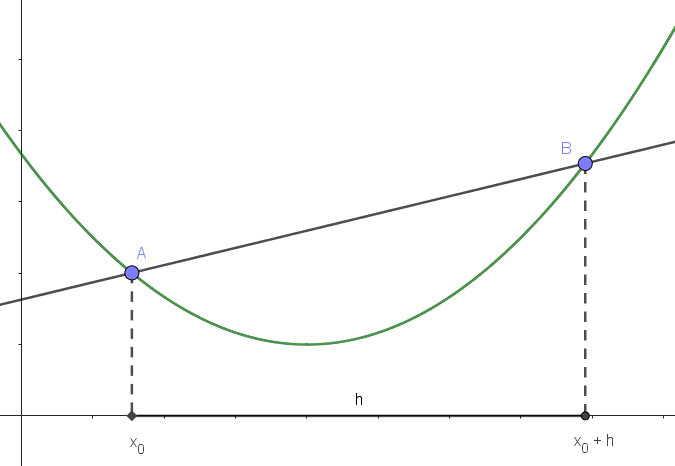
\includegraphics[width=0.35\textwidth]{slike/odvod1.png}
    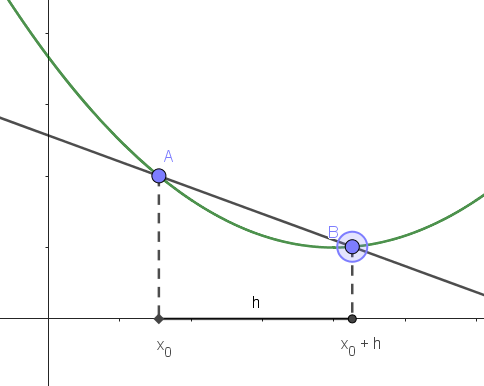
\includegraphics[width=0.3\textwidth]{slike/odvod2.png}
    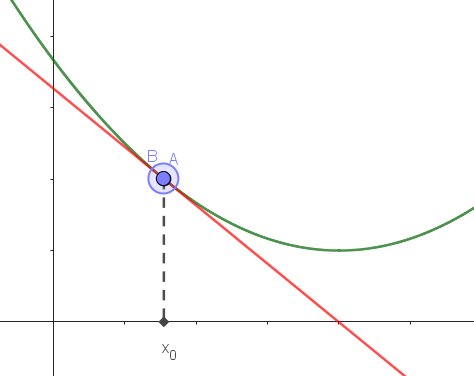
\includegraphics[width=0.32\textwidth]{slike/odvod3.png}
\end{figure*}

\didopomba{Ustno povemo idejo tangente -- točko, v kateri jo želimo, fiksiramo, si izberemo eno drugo točko, potegnemo skozi sekanto in točko približujemo prvi. Vidimo, da dobimo res tangento.}

Zapišimo koeficient sekante: $ \frac{f(x_0 + h) - f(x_0)}{(x_0 + h) - x_0} = \frac{f(x_0 + h) - f(x_0)}{h} $. Tangento dobimo, ko gre $ h $ proti $ 0 $ \didopomba{To NI, da vstaviš $ h = 0 $, ker dobiš $ \frac{0}{0} $, zato vzameš limito (spomnimo se limite $ \frac{\sin x}{x} $)}

Koeficient tangente na $ f $ v točki $ x_0 $ je \didopomba{najprej zapiši limito in nato šele uvedi rdečo oznako}
$$ \textcolor{red}{f'(x_0) = } \lim_{h \to 0} \frac{f(x_0 + h) - f(x_0)}{h} $$

\didopomba{Sedaj pa še ime za to oznako:}

\textbf{Odvod} funkcije v dani točki je smerni koeficient tangente na funkcijo v tej točki: $ k_t = f(x_0) $.

\vaje{Vaja:
\begin{itemize}
    \item Izračunaj splošen odvod funkcije $ f(x) = 3x + 2 $ in $ g(x) = 8 $ \didopomba{tukaj najprej razberejo odvod iz grafa (odvod premice kar koeficient premice, odvod konstante je 0, ker je to itak vodoravna premica), nato pa se prepričajo še računsko} \\
    \textcolor{red}{$ \lim_{h \to 0} c = 0 $}
    \item Zapiši koeficient tangente na graf funkcije $ f(x) = x^2 $ v točki $ x = 2 $ in $ x = - 3 $ \didopomba{najprej slikca, narišemo približno tangento in ugotavljamo, koliko prb. bi bil koeficient. Bistveno, da je v $ -3 $ negativen in v 2 pozitiven}. Splošen koeficient: \\
    $ f'(x) = \lim_{h \to 0} \frac{f(x + h) - f(x)}{h} = \lim_{h \to 0} \frac{(x + h)^2 - x^2}{h} = \lim_{h \to 0} \frac{2hx + h^2}{h} = \lim_{h \to 0} 2x + h = 2x $ \\
    Narišeš slikco grafa odvoda in primerjaš z grafom $ f $. Odvod je negativen točno tam, kjer je tangenta ``padajoča''
    $ k(2) = 4, k(-3) = -6 $
\end{itemize}
}

PRAVILA: \didopomba{lahko dokažemo ta prvo, potem pa naj ostale npr. za DN ali pa sam pogledajo v učbenik, ne bi zgubljali časa s tem}
\begin{itemize}
    \item $ (f \pm g)'(x) = f'(x) \pm g'(x) $
    \item $ (f \cdot g)'(x) = f'(x)g(x) + f(x)g'(x) $
    \item $ (k \cdot f)'(x) = k \cdot f'(x) $
    \item $ \left( \frac{1}{f} \right)'(x) = - \frac{f'(x)}{f^2(x)} $
    \item $ \left( \frac{f}{g} \right)'(x) = \frac{f'(x)g(x) - f(x)g'(x)}{g^2(x)} $
\end{itemize}

\newpage

\didopomba{izračunamo te tri primere po definiciji (drugega smo že pri vaji)}

$ x' = 1 \\
(x^2)' = 2x \\
(x^3)' = 3x^2 $ \didopomba{Tu se že kar namatramo, zato uporabimo pravilo produkta} $ (x^3)' = (x \cdot x^2)' = x^2 + x \cdot 2x = 3x^2 $

Za splošen $ n : \textcolor{red}{(x^n)' = n \cdot x^{n - 1}} $.
\begin{itemize}
    \item $ n \in \mathbb{N} $ -- dokažemo z indukcijo na $ n $:

    Za $ n = 1 $ očitno velja. IP: $ (x^n)' = n \cdot x^{n - 1} $, dokazujemo za $ n + 1 $:
    
    $ (x^{n + 1})' = (x \cdot x^n)' = x' \cdot x^n + x \cdot (x^n)' = x^n + x \cdot n \cdot x^{n - 1} = x^n + n \cdot x^n = (n + 1) x^n $

    \item Kaj pa $ (x^{-n})' $, kjer je $ n \in \mathbb{N} $? Zapišemo $ x^{-n} = \frac{1}{x^{n}} $ in upoštevamo pravilo odvoda obratne funkcije: $ (x^{-n})' = \left( \frac{1}{x^{n}} \right)' = - \frac{(x^n)'}{x^{2n}} = - \frac{n \cdot x^{n - 1}}{x^{2n}} = - n \cdot x^{-n - 1} $
    \item izkaže se, da formula velja za vsak $ n \in \mathbb{R} $ \didopomba{gl. učbenik, ne bomo mi dokazovali}
\end{itemize} 


\vaje{
Vaje:
\begin{itemize}
    \item Drug zapis definicije odvoda:
        \subitem $ f'(x) = \lim_{h \to 0} \frac{f(x) - f(x - h)}{h} $
        \subitem $ f'(x) = \lim_{x_2 \to x_1} \frac{f(x_2) - f(x_1)}{x_2 - x_1} $
        \subitem $ \lim_{h \to 0} \frac{f(x) - f(x + h)}{h} = - f(x_0) $ \ldots
    \item Basic vaje iz odvodov elementarnih funkcij
\end{itemize}
}
    
\end{priprava}